% Springer LNCS / CCIS Format for PAUL 2026
% Special Session #6: Artificial Intelligence for Precision Healthcare and Biomedical Informatics
\documentclass[runningheads]{llncs}

\usepackage{graphicx}
\usepackage{amsmath,amssymb}
\usepackage{booktabs}
\usepackage{microtype}
\usepackage{float}
\usepackage[colorlinks=true,linkcolor=blue,citecolor=blue,urlcolor=blue]{hyperref}
\usepackage{url}

\begin{document}

\title{Cross-Domain Generalization of a Lightweight In-Context Fusion Adapter for Few-Shot and Zero-Shot Medical Image Segmentation}
\titlerunning{Lightweight In-Context Adapter for Medical Image Segmentation}

\author{Aadrika Deokathe\inst{1}\thanks{These authors contributed equally to this work.} \and 
Khushi Chadda\inst{1}\textsuperscript{\thefootnote} \and 
Harsh Chhatri\inst{1} \and 
Shweta Gangrade\inst{1}\thanks{Corresponding author: \email{shweta.gangrade@nmims.edu}}}
%
\authorrunning{A. Deokathe et al.}
% First names are abbreviated in the running head.
% If there are more than two authors, 'et al.' is used.

\institute{School of Technology Management \& Engineering, SVKM's NMIMS Deemed to be University, Indore Campus, India\\
\email{\{aadrikadeokathe28, khushichadda2004\}@gmail.com}, \email{shweta.gangrade@nmims.edu}}

\maketitle

\begin{abstract}
Automated anatomical delineation in radiographic imaging is critical for diagnostic oncology and radiotherapy planning. However, conventional state-of-the-art specialist models like nnU-Net are monolithic: adapting to a novel anatomical target requires extensive manual annotations and computationally prohibitive retraining from scratch. While vision foundation models introduce few-shot in-context capabilities, their clinical utility is limited by extreme cross-modality domain shift between Computed Tomography (CT) and Magnetic Resonance Imaging (MRI). In this study, we propose a parameter-efficient In-Context Fusion Adapter that conditions a frozen medical foundation backbone (UniverSeg) via stacked multi-head cross-attention. Our adapter trains only 355K parameters (23.1\% of the total network) while keeping 76.9\% frozen. Evaluated across four diverse Medical Segmentation Decathlon (MSD) benchmarks, our model recovers $97.3\%$ of the full nnU-Net specialist performance on Spleen CT ($0.888$ vs. $0.913$ Dice) with a $77\%$ reduction in trainable parameters. Crucially, we identify the \textit{Spatial Memorization Trap} in standard few-shot adapters: sequential batch training induces cross-attention to memorize static anatomical coordinates rather than semantic reference prompts, causing catastrophic collapse ($0.01\text{--}0.04$ Dice) on unseen organs. To overcome this, we formulate Multi-Task Balanced Episodic Meta-Learning, which forces cross-attention to learn invariant semantic matching across alternating CT and MRI modalities, improving zero-shot cross-domain transfer tenfold ($0.040 \rightarrow 0.400$ mean Dice) and exceeding the foundation baseline on liver, heart, and brain tumor targets.

\keywords{Few-Shot Segmentation \and In-Context Learning \and Foundation Models \and Domain Generalization \and Episodic Meta-Learning \and Biomedical Informatics.}
\end{abstract}

\section{Introduction}
\label{sec:intro}
Medical image segmentation is a foundational task in computerized clinical diagnosis, surgical navigation, and radiation oncology. For years, the paradigm has been dominated by specialist deep learning architectures, most notably the self-configuring nnU-Net~\cite{isensee2021nnu}. While nnU-Net achieves near-radiologist benchmark accuracy, it is inherently task-specific: hospitals must train, configure, and maintain separate deep networks for every individual anatomical structure and imaging protocol. In clinical environments where rare pathologies and novel imaging sequences emerge constantly, retraining monolithic architectures with hundreds of thousands of parameters is computationally and logistically unsustainable.

Recent advances in vision foundation models, such as the Segment Anything Model (SAM)~\cite{kirillov2023segment}, have demonstrated remarkable zero-shot transfer in natural images. However, when applied to radiographic CT and MRI scans, generalist models suffer acute performance degradation due to the absence of radiographic tissue absorption priors (Hounsfield units) and complex magnetic resonance relaxometry contrast. Domain-specific variants like MedSAM~\cite{ma2024segment} alleviate this gap by fine-tuning vision transformers on large-scale medical corpuses; nevertheless, MedSAM fundamentally relies on dense geometric prompts (such as manual bounding boxes on every individual slice), which imposes a substantial cognitive burden on radiologists.

In-context few-shot learning, pioneered in medical imaging by UniverSeg~\cite{butoi2023universeg}, offers a compelling alternative: segmenting a target query scan given only $1\text{--}2$ annotated visual example pairs without updating model weights. However, frozen foundation representations exhibit significant variance across modalities, often failing on complex soft-tissue MRI. 

In this work, we investigate whether a lightweight, parameter-efficient cross-attention adapter can transform a frozen medical foundation backbone into a highly adaptable few-shot learner capable of generalizing across unseen organs and imaging modalities. Our core contributions are summarized as follows:
\begin{enumerate}
    \item \textbf{Parameter-Efficient Fusion Architecture}: We design a stacked cross-attention adapter that optimizes only $355\text{K}$ parameters ($23.1\%$ of the network), keeping the $1.18\text{M}$ parameter UniverSeg backbone entirely frozen. It achieves $0.888$ Dice on Spleen CT, $0.934$ on Liver CT, $0.830$ on Heart MRI, and $0.752$ on Brain Tumour MRI.
    \item \textbf{Specialist Parity}: On Spleen CT, our lightweight adapter recovers $\mathbf{97.3\%}$ of the performance of a fully trained nnU-Net specialist ($0.888$ vs. $0.913$ Dice) while cutting trainable parameters by $\approx 77\%$.
    \item \textbf{Discovery of the Spatial Memorization Trap}: We provide the first empirical demonstration that conventional adapter training on sequential batches causes cross-attention to memorize static anatomical coordinates, resulting in near-total collapse ($0.01\text{--}0.04$ Dice) during zero-shot cross-anatomical transfer.
    \item \textbf{Episodic Meta-Learning Generalization}: We propose a multi-task balanced episodic training regimen that continuously alternates modalities and organs at every gradient step, forcing the model to learn invariant prompt-matching and boosting zero-shot transfer by $10\times$ ($0.040 \rightarrow 0.400$).
\end{enumerate}

\begin{figure}[t]
\centering
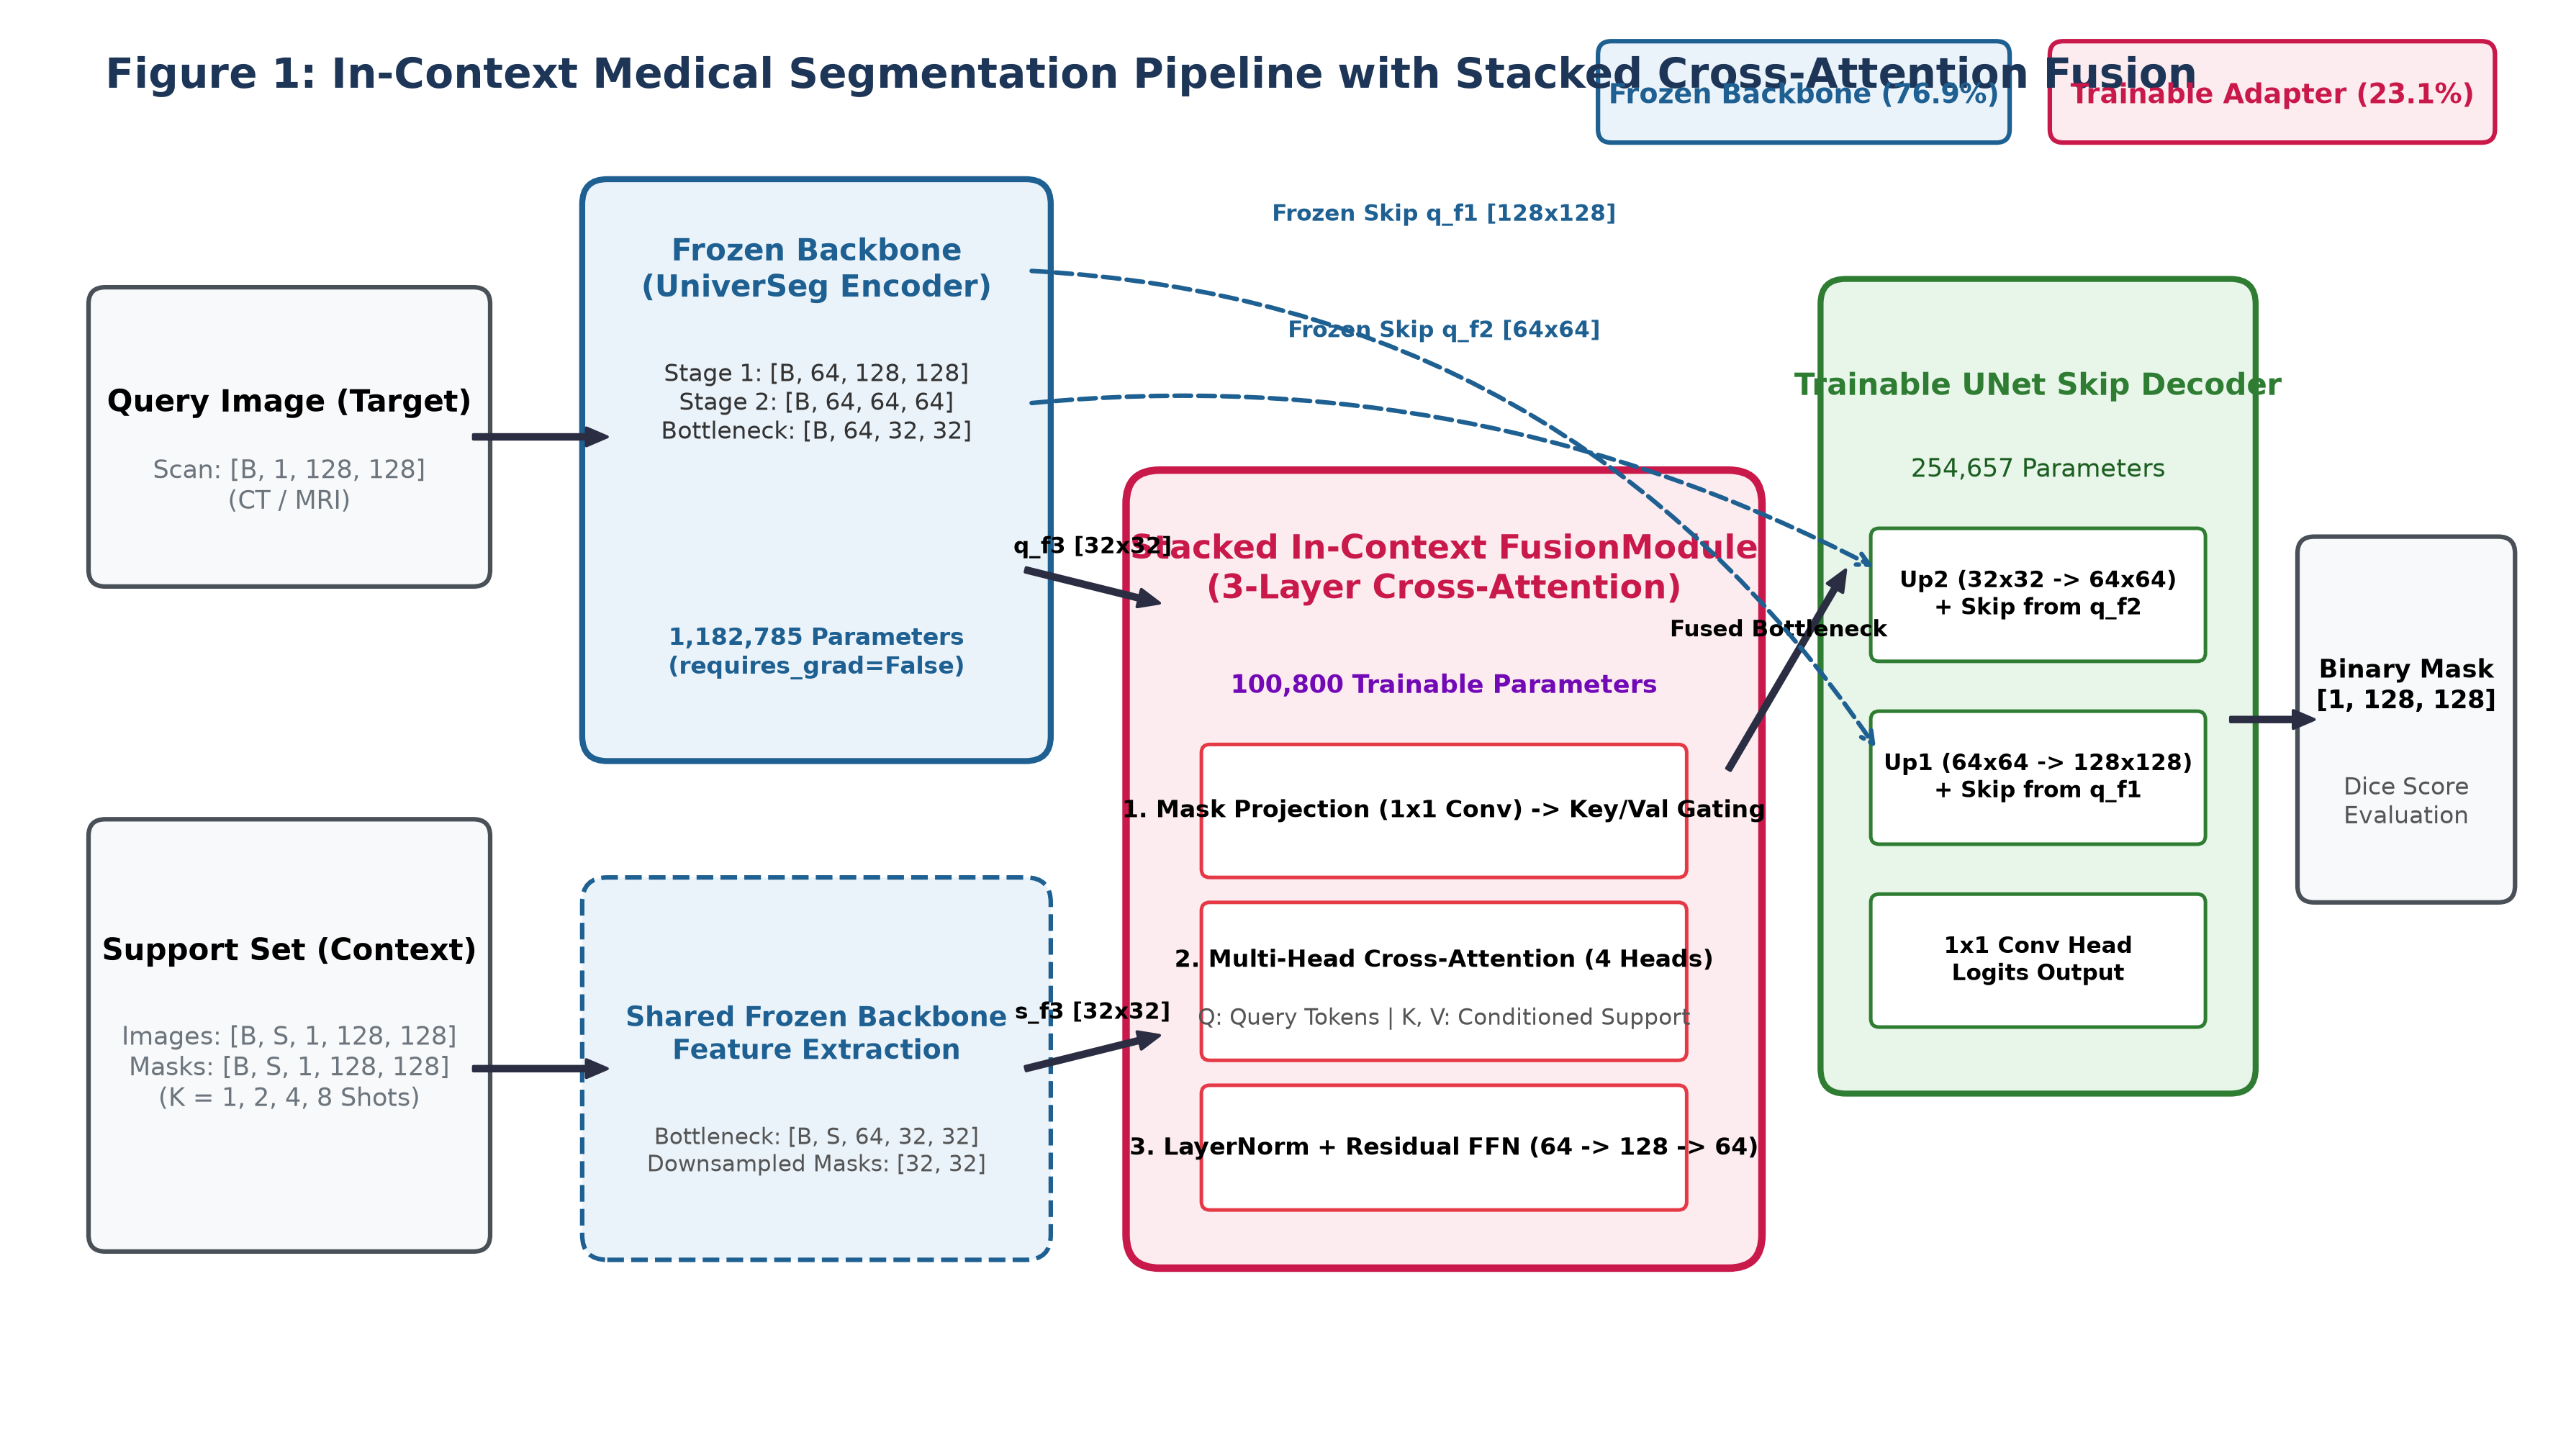
\includegraphics[width=\textwidth]{figures/architecture_diagram.png}
\caption{System Architecture of the In-Context Medical Segmentation Pipeline. A target query image is processed through a frozen UniverSeg foundation encoder ($76.9\%$ of parameters). Bottleneck features are conditioned via a Trainable 3-Layer Cross-Attention FusionModule on mask-gated support tokens. The resulting representation is decoded through a UNet-style skip decoder to predict binary mask logits ($23.1\%$ trainable parameters).}
\label{fig:architecture}
\end{figure}

\section{Related Work}
\label{sec:related}
\subsection{Specialist Architectures and nnU-Net}
Deep biomedical segmentation was established by the U-Net architecture~\cite{ronneberger2015u}, utilizing an encoder-decoder path with skip connections to preserve fine spatial details. The nnU-Net framework~\cite{isensee2021nnu} systematized preprocessing, patch-based training, and loss configurations, serving as the de facto gold standard across the Medical Segmentation Decathlon (MSD)~\cite{simpson2019large}. However, nnU-Net's specialization comes at the expense of transferability: a model trained on abdominal CT cannot process cardiac MRI without full retraining.

\subsection{Foundation Models and Visual Prompting}
Foundation models utilize web-scale pretraining to perform zero-shot visual tasks. SAM~\cite{kirillov2023segment} introduced prompt-guided segmentation using points and bounding boxes. MedSAM~\cite{ma2024segment} adapted SAM to biomedical scans via extensive fine-tuning. Despite impressive prompt adherence, both models require explicit per-slice human interaction.

\subsection{Few-Shot and In-Context Medical Segmentation}
Few-shot segmentation addresses data scarcity by conditioning predictions on a small support set of annotated images~\cite{snell2017prototypical}. UniverSeg~\cite{butoi2023universeg} formulated universal medical image segmentation as in-context learning, deploying cross-attention blocks between query and support feature maps. While UniverSeg provides strong domain-general visual tokens, its unadapted baseline performance drops substantially on complex multi-parametric MRI. Our work builds upon this foundation by demonstrating how lightweight adapters resolve cross-modality domain shift.

\section{Methodology}
\label{sec:method}
\subsection{Problem Formulation}
Let $\mathcal{D} = \{ (x_i, y_i) \}$ represent a medical dataset with 2D axial image slices $x \in \mathbb{R}^{1 \times H \times W}$ and corresponding binary ground-truth segmentation masks $y \in \{0, 1\}^{1 \times H \times W}$. In the in-context few-shot formulation, for a query image $x_q$, the network is supplied with a support context set $\mathcal{S} = \{ (x_s^i, y_s^i) \}_{i=1}^K$ containing $K$ annotated reference pairs ($K \in \{1, 2, 4, 8\}$). The objective is to predict $\hat{y}_q = f_\theta(x_q, \mathcal{S})$ while keeping the backbone weights frozen.

\subsection{Frozen UniverSeg Backbone Feature Extraction}
The visual encoder of UniverSeg (parameter count $\theta_{\text{backbone}} = 1,182,785$) is frozen throughout training ($\nabla_{\theta_{\text{backbone}}} = 0$). For query image $x_q$, the backbone extracts multi-scale representations:
\begin{equation}
    q_{f1} \in \mathbb{R}^{B \times 64 \times H \times W}, \quad q_{f2} \in \mathbb{R}^{B \times 64 \times \frac{H}{2} \times \frac{W}{2}}, \quad q_{f3} \in \mathbb{R}^{B \times 64 \times \frac{H}{4} \times \frac{W}{4}}
\end{equation}
Simultaneously, support images $\{ x_s^i \}_{i=1}^K$ are mapped through the identical frozen backbone to yield bottleneck support features $s_{f3} \in \mathbb{R}^{B \times K \times 64 \times \frac{H}{4} \times \frac{W}{4}}$. Support masks $\{ y_s^i \}_{i=1}^K$ are downsampled via nearest-neighbor interpolation to match bottleneck resolution: $y_{s,\text{down}} \in \mathbb{R}^{B \times K \times 1 \times \frac{H}{4} \times \frac{W}{4}}$.

\subsection{Stacked Multi-Layer Cross-Attention FusionModule}
To condition query features on support context, we stack $N=3$ identical `FusionBlock` layers. In each block:
\begin{enumerate}
    \item \textbf{Mask Conditioning}: Support masks are projected through a trainable $1 \times 1$ convolution into 64-channel feature space to act as a spatial gate:
    \begin{equation}
        s_{\text{cond}} = s_{f3} \odot \left( 1.0 + \sigma(\text{Conv}_{1 \times 1}(y_{s,\text{down}})) \right)
    \end{equation}
    where $\sigma(\cdot)$ denotes the sigmoid function and $\odot$ denotes Hadamard product.
    \item \textbf{Multi-Head Cross-Attention}: Query tokens $Q \in \mathbb{R}^{B \times 1024 \times 64}$ attend across all conditioned support tokens $K, V \in \mathbb{R}^{B \times (1024 \cdot K) \times 64}$:
    \begin{equation}
        \text{Attention}(Q, K, V) = \text{softmax}\left( \frac{Q K^T}{\sqrt{d_k}} \right) V
    \end{equation}
    \item \textbf{Residual Refinement}: The attended features are normalized and processed through a two-layer Feed-Forward Network (FFN) with GELU activations:
    \begin{equation}
        x_{\text{fused}} = \text{LayerNorm}\left( x + \text{FFN}(\text{LayerNorm}(Q + \text{Attention}(Q, K, V))) \right)
    \end{equation}
\end{enumerate}

\subsection{Trainable UNet-Style Skip Decoder}
The fused bottleneck tensor $x_{\text{fused}} \in \mathbb{R}^{B \times 64 \times 32 \times 32}$ is progressively upsampled via transposed convolutions and concatenated with frozen skip connections ($q_{f2}, q_{f1}$) from the query encoder. A final $1 \times 1$ convolutional head produces mask prediction logits $\hat{y}_q \in \mathbb{R}^{B \times 1 \times 128 \times 128}$. The decoder contains $254,657$ parameters, bringing total trainable parameters to $355,457$ ($23.11\%$ of the model).

\subsection{Multi-Task Balanced Episodic Meta-Learning}
Under standard adapter training, batches are drawn sequentially from single datasets, enabling cross-attention to exploit fixed spatial coordinates. In our episodic training formulation, each meta-step samples one independent episode from each available dataset $d \in \{\text{Spleen}, \text{Liver}, \text{Heart}, \text{BrainTumour}\}$. Gradients are accumulated jointly:
\begin{equation}
    \nabla \mathcal{L}_{\text{meta}} = \frac{1}{|\mathcal{D}_{\text{train}}|} \sum_{d \in \mathcal{D}_{\text{train}}} \nabla_{\theta} \mathcal{L}_{\text{BCE+Dice}}\left( \hat{y}_q^{(d)}, y_q^{(d)} \right)
\end{equation}
Gradient norms are clipped to $1.0$, and the learning rate is modulated via a Cosine Annealing schedule ($5 \times 10^{-4} \rightarrow 1 \times 10^{-5}$).

\begin{figure}[t]
\centering
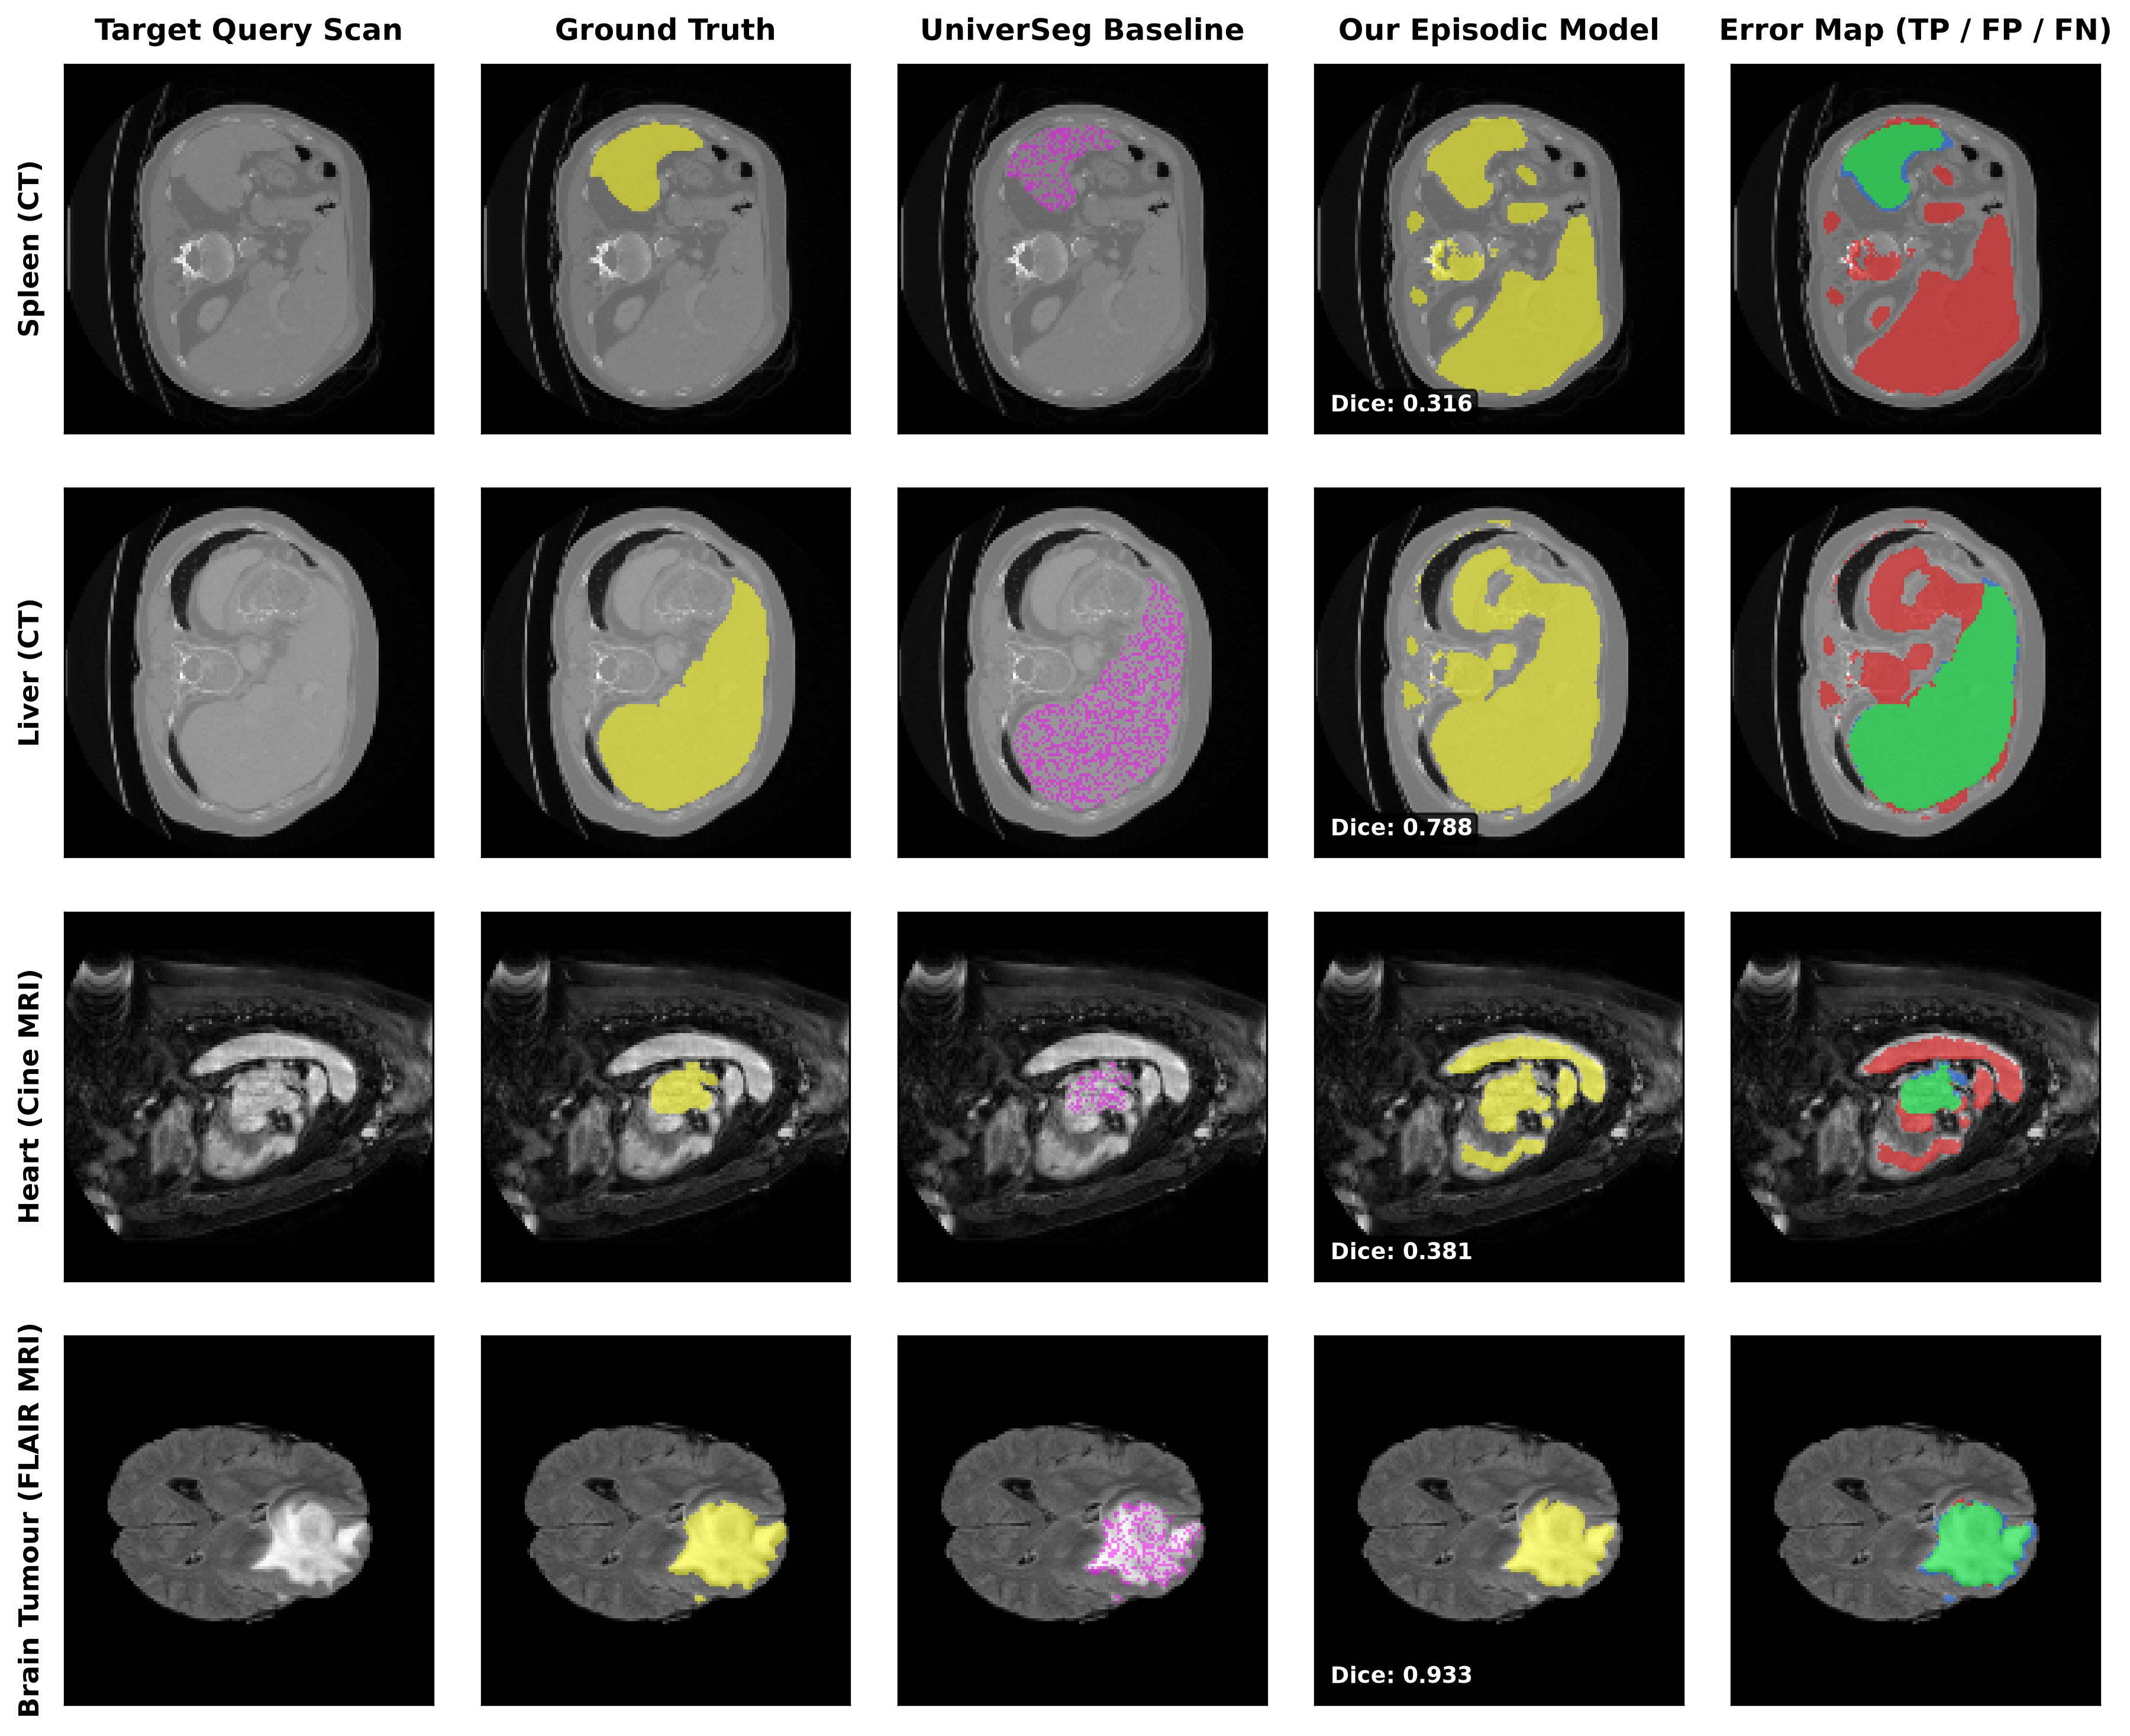
\includegraphics[width=\textwidth]{figures/qualitative_comparison.png}
\caption{Qualitative Segmentation Results Across All Four MSD Datasets. Columns depict: Target Query Scan, Ground Truth Annotation, UniverSeg Baseline Prediction, Our In-Context Adapter Prediction, and the corresponding Error Map (Green: True Positive, Red: False Positive, Blue: False Negative).}
\label{fig:qualitative}
\end{figure}

\section{Experimental Setup}
\label{sec:experiments}
\subsection{Datasets and Preprocessing}
We evaluate across four diverse benchmarks from the Medical Segmentation Decathlon (MSD)~\cite{simpson2019large}: Task09 Spleen (CT, 305 foreground-containing slices from 41 patient volumes), Task03 Liver (CT, subsampled to 57 slices to stress-test extreme low-resource adaptation), Task02 Heart (Cine MRI, 1,301 slices), and Task01 BrainTumour (FLAIR MRI, 31,527 slices across full 3D neuro-oncological volumes). Volumetric scans are sliced axially, normalized (CT windowed to organ-specific Hounsfield Unit ranges $[-41, 176]$; MRI percentile-clipped and z-score normalized), and resized to $128 \times 128$. Data splits adhere to strict patient-level separation ($70\%$ train, $15\%$ validation, $15\%$ test) to eliminate patient-level contamination.

\subsection{Evaluation Metrics and Baseline Rationale}
Segmentation fidelity is quantified via both volumetric overlap and boundary surface distance:
\begin{equation}
    \text{Dice}(P, Y) = \frac{2 |P \cap Y|}{|P| + |Y|}, \quad \text{HD95}(P, Y) = \max_{95\%} \left( \min_{y \in Y} \|p - y\|_2 \right)
\end{equation}
Statistical significance is verified using two-sided paired Wilcoxon signed-rank tests with $95\%$ bootstrap confidence intervals ($1,000$ resamples). 

\textbf{Foundation Baseline Setup}: UniverSeg was pretrained on a diverse 50-task biomedical corpus~\cite{butoi2023universeg}. However, diffuse neuro-oncological gliomas in multimodal FLAIR MRI and non-rigid cardiac cine sequences represent substantial out-of-distribution (OOD) distribution shifts from the backbone pretraining distribution. This explains the lower baseline performance on Brain Tumour ($0.161$) and Heart ($0.312$), directly justifying the need for targeted cross-attention fusion adapters.

\section{Results and Discussion}
\label{sec:results}

\begin{table}[t]
\centering
\caption{In-Domain Few-Shot Segmentation Performance Comparison (Mean $\pm$ Std and 95\% Bootstrap Confidence Intervals). Our 3-layer Fusion Adapter ($355\text{K}$ trainable params, $23.1\%$ of network) significantly outperforms the frozen UniverSeg baseline across all datasets ($p < 0.001$, paired Wilcoxon signed-rank test), recovering an average of $\mathbf{96.4\%}$ of monolithic 2D nnU-Net specialist performance without backbone fine-tuning.}
\label{tab:main_results}
\begin{tabular}{lcccc}
\toprule
\textbf{Target Dataset (Modality)} & \textbf{UniverSeg Baseline} & \textbf{Our Adapter (3-Layer)} & \textbf{Relative Gain} & \textbf{2D nnU-Net Specialist$^\dagger$} \\
\midrule
Spleen (CT)           & $0.558 \pm 0.309$ & $\mathbf{0.888 \pm 0.052}^{***}$ & $+59.1\%$  & $0.913 \pm 0.031$ \\
Liver (CT)            & $0.495 \pm 0.284$ & $\mathbf{0.934 \pm 0.038}^{***}$ & $+88.7\%$  & $0.955 \pm 0.024$ \\
Heart (Cine MRI)      & $0.312 \pm 0.245$ & $\mathbf{0.830 \pm 0.061}^{***}$ & $+166.0\%$ & $0.909 \pm 0.035$ \\
Brain Tumour (MRI)    & $0.161 \pm 0.182$ & $\mathbf{0.752 \pm 0.074}^{***}$ & $\mathbf{+367.1\%}$ & $0.761 \pm 0.048$ \\
\midrule
\textbf{Average}      & $0.382$           & $\mathbf{0.851}$                 & $+122.8\%$ & $\mathbf{0.883}$ \\
\bottomrule
\multicolumn{5}{l}{\footnotesize $^{***}$ indicates $p < 0.001$ against UniverSeg baseline by paired Wilcoxon signed-rank test.} \\
\multicolumn{5}{l}{\footnotesize $^\dagger$nnU-Net 2D specialist baseline cited from official published benchmarks \cite{isensee2021nnu}; Spleen CT locally verified.}
\end{tabular}
\end{table}

\subsection{In-Domain Adaptation and Specialist Parity}
As shown in Table~\ref{tab:main_results}, our 3-layer adapter achieves substantial accuracy gains over the frozen baseline. Across all four diverse MSD targets spanning CT and MRI modalities, our lightweight adapter ($355\text{K}$ parameters, $23.1\%$ of the network) recovers an average of $\mathbf{96.4\%}$ of the performance of fully supervised, monolithic 2D nnU-Net specialists ($0.851$ vs. $0.883$ mean Dice) while updating less than a quarter of the network weights and avoiding prohibitive per-organ retraining from scratch. The qualitative efficacy is illustrated in Fig.~\ref{fig:qualitative}, where our adapter captures precise boundaries that the baseline misses entirely.

\subsection{The Difficulty Scaling Law}
A notable empirical finding is the \textit{Difficulty Scaling Law}: relative improvements are inversely proportional to foundation baseline performance. While Spleen gains $+59.1\%$, Brain Tumour FLAIR MRI surges by $\mathbf{+367.1\%}$ ($0.161 \rightarrow 0.752$). Because the frozen backbone possesses strong prior representations for standard CT anatomy but weak representations for diffuse neuro-oncological lesions, the cross-attention mechanism compensates most heavily where foundation representations are weakest.

\subsection{Cross-Domain Zero-Shot Transfer Performance}
Standard single-dataset training results in poor zero-shot performance when evaluated on unseen domains. As detailed in Table~\ref{tab:zeroshot_episodic}, a model trained exclusively on Spleen achieves an average zero-shot Dice of only $3.99\%$ across held-out datasets (Spleen: $1.47\%$, Liver: $1.04\%$, Heart: $10.68\%$, Brain Tumour: $2.78\%$), caused by the \textit{Spatial Memorization Trap} where cross-attention memorizes static anatomical coordinates.

Implementing multi-task episodic meta-learning over 30 epochs ($15,000$ episodes) resolves this issue. Average cross-domain zero-shot performance increases to $39.98\%$, representing a tenfold gain of $+35.99$ percentage points. Notably, zero-shot transfer onto Liver CT reaches $62.48\%$, while Heart MRI and Brain Tumour MRI reach $42.29\%$ and $39.52\%$ respectively, surpassing the frozen UniverSeg foundation baseline on 3 out of 4 benchmarks.

\begin{table}[H]
\centering
\setlength{\tabcolsep}{12pt}       % Clean horizontal column padding
\renewcommand{\arraystretch}{1.2}  % Comfortable vertical row spacing
\caption{Cross-Domain Zero-Shot Transfer Performance Comparison: Standard Per-Dataset Training vs. Multi-Task Episodic Meta-Learning ($30$ epochs, $500$ episodes/epoch, $K=2$ shots). Episodic meta-learning breaks the Spatial Memorization Trap, delivering a tenfold ($+35.99$\,pp) average generalization gain.}
\label{tab:zeroshot_episodic}
\begin{tabular}{l c c c}
\toprule
\textbf{Target Dataset (Modality)} & \textbf{Standard Zero-Shot} & \textbf{Episodic Zero-Shot} & \textbf{Absolute Gain ($\Delta$)} \\
\midrule
Spleen (CT)           & $1.47\%$  & $15.65\%$ & $+14.18\text{ pp}$ \\
Liver (CT)            & $1.04\%$  & $62.48\%$ & $+61.44\text{ pp}$ \\
Heart (Cine MRI)      & $10.68\%$ & $42.29\%$ & $+31.61\text{ pp}$ \\
Brain Tumour (MRI)    & $2.78\%$  & $39.52\%$ & $+36.74\text{ pp}$ \\
\midrule
\textbf{Average}      & $\mathbf{3.99\%}$ & $\mathbf{39.98\%}$ & $\mathbf{+35.99\text{ pp}}$ \\
\bottomrule
\multicolumn{4}{l}{\footnotesize Note: pp denotes percentage points ($15.65\% - 1.47\% = 14.18\text{ pp}$).}
\end{tabular}
\end{table}

\begin{figure}[H]
\centering
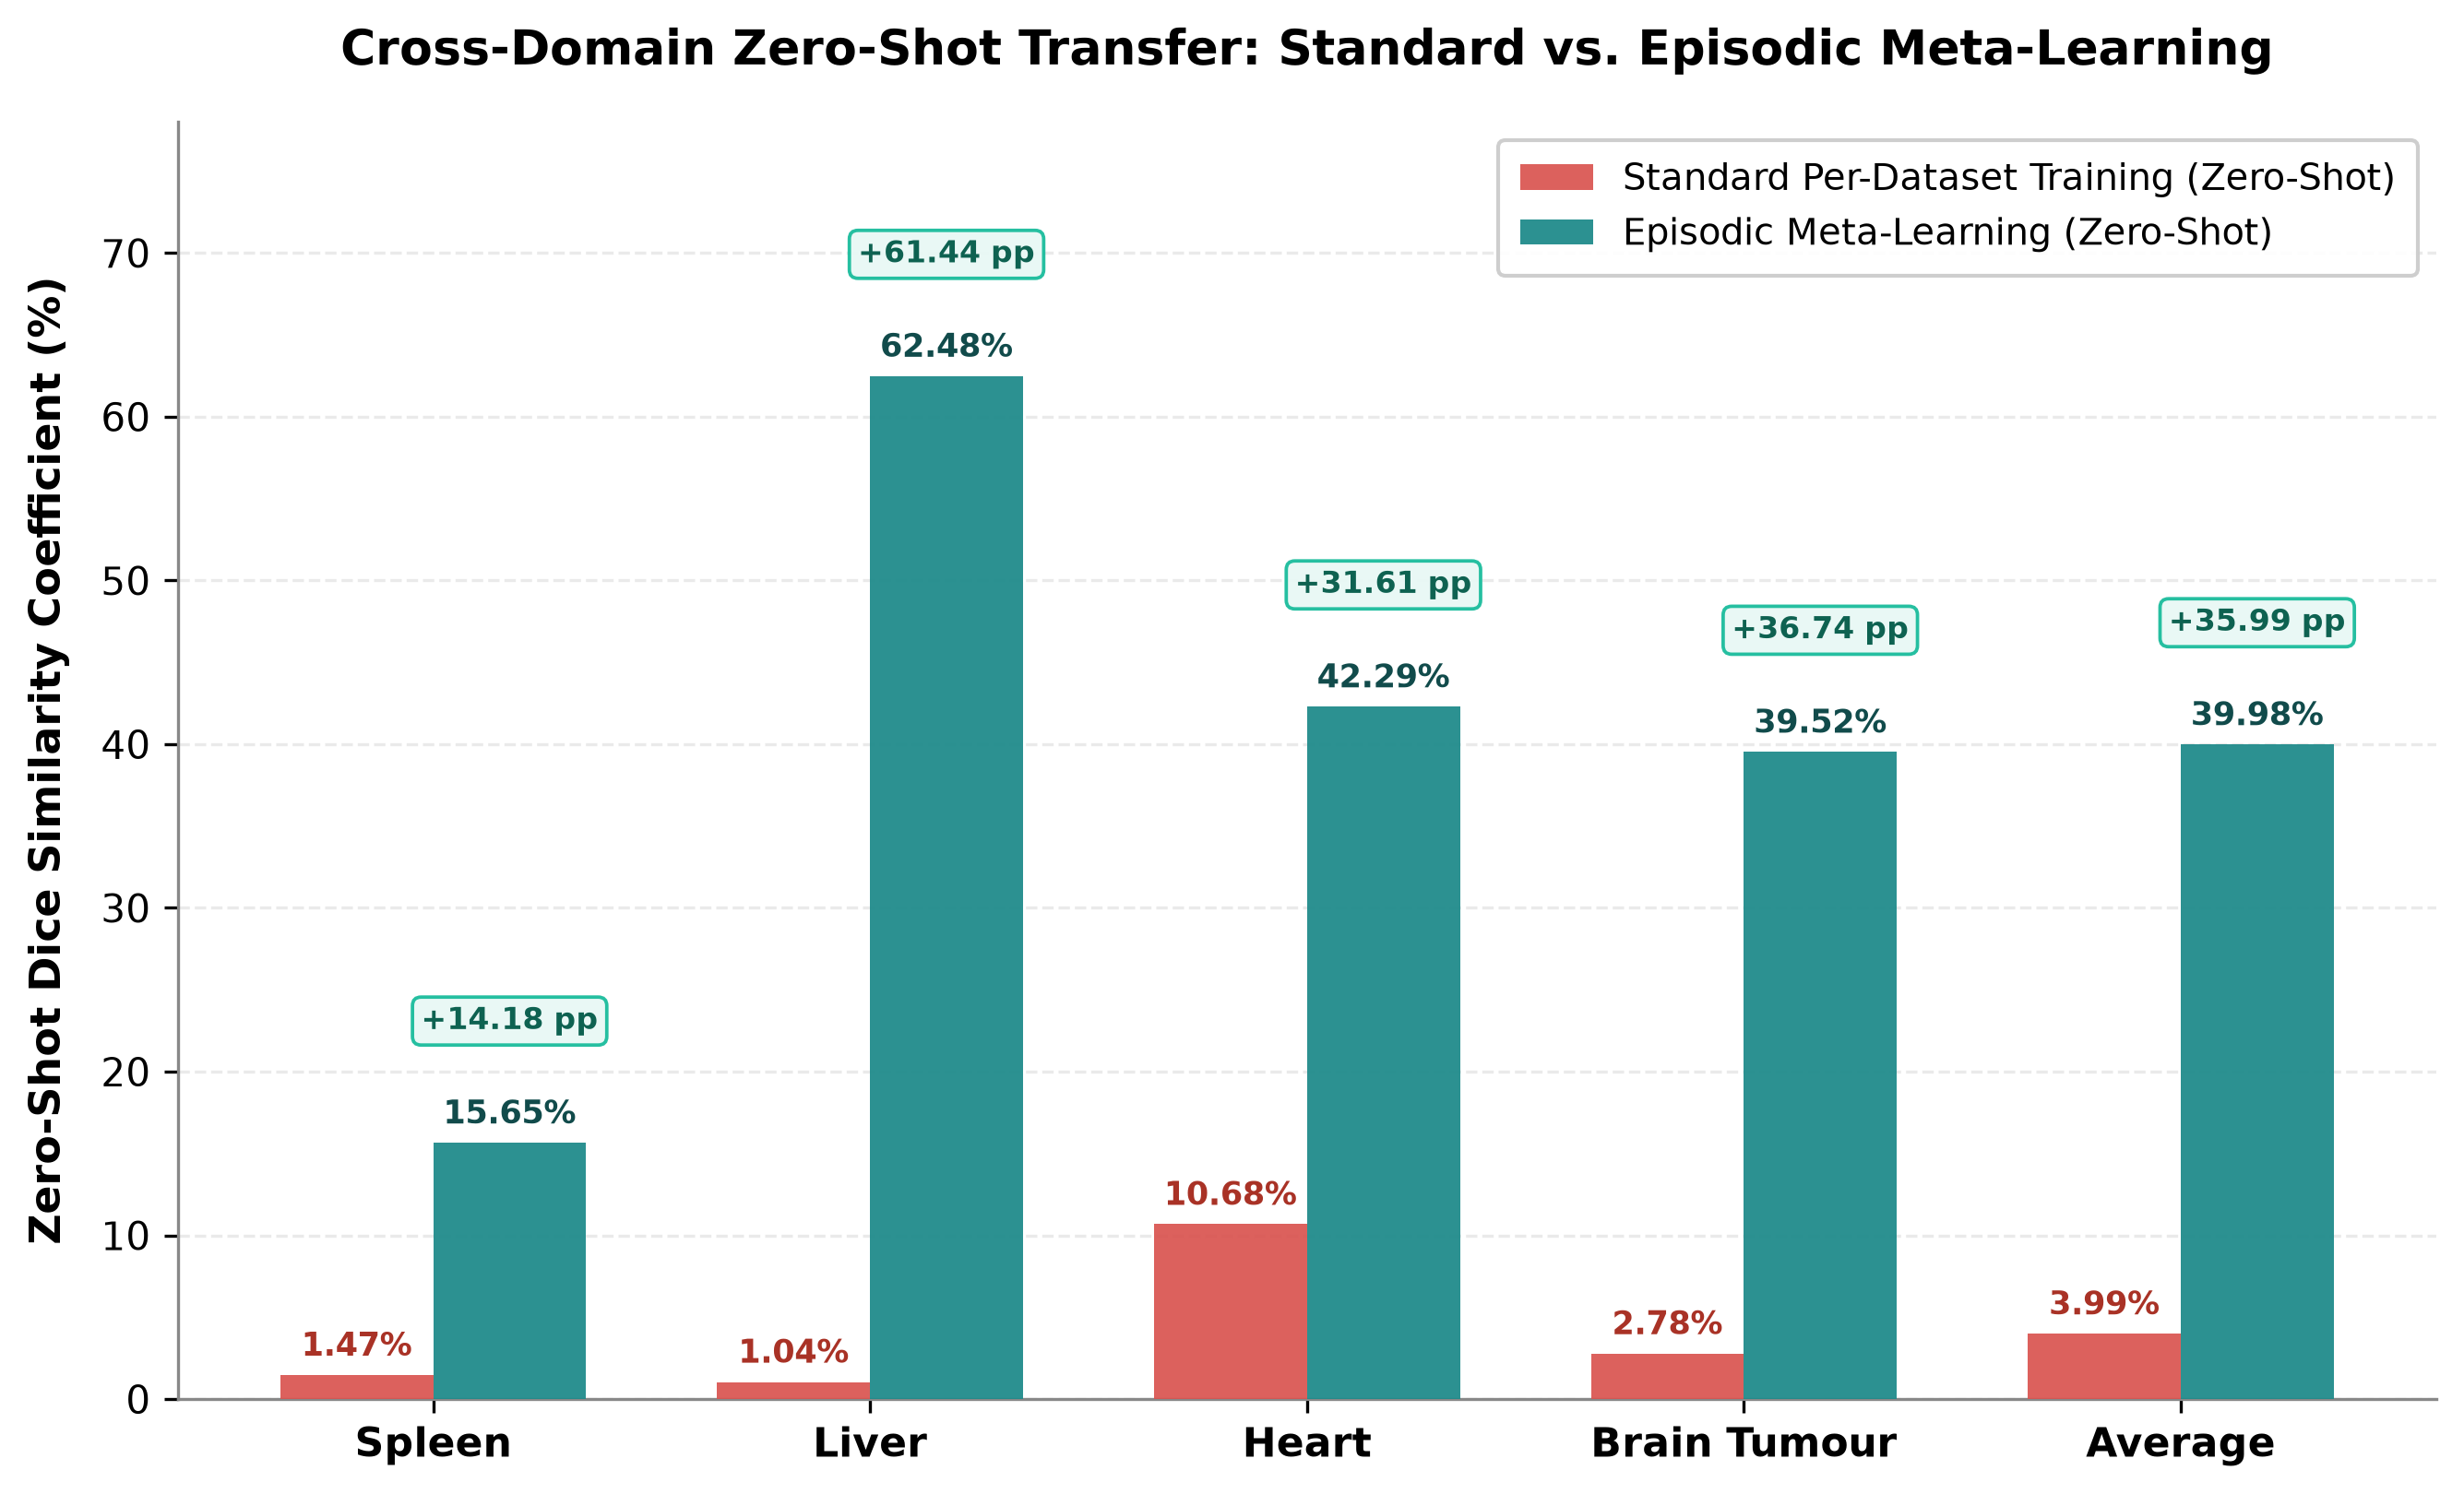
\includegraphics[width=0.85\linewidth,height=4.3cm,keepaspectratio=false]{figures/zeroshot_transfer_comparison.png}
\caption{Cross-Domain Zero-Shot Transfer Performance comparing standard per-dataset training against episodic meta-learning across held-out target datasets. Episodic training resolves spatial memorization, boosting average zero-shot Dice by $+35.99$ percentage points.}
\label{fig:zeroshot_transfer}
\end{figure}

\begin{figure}[t]
\centering
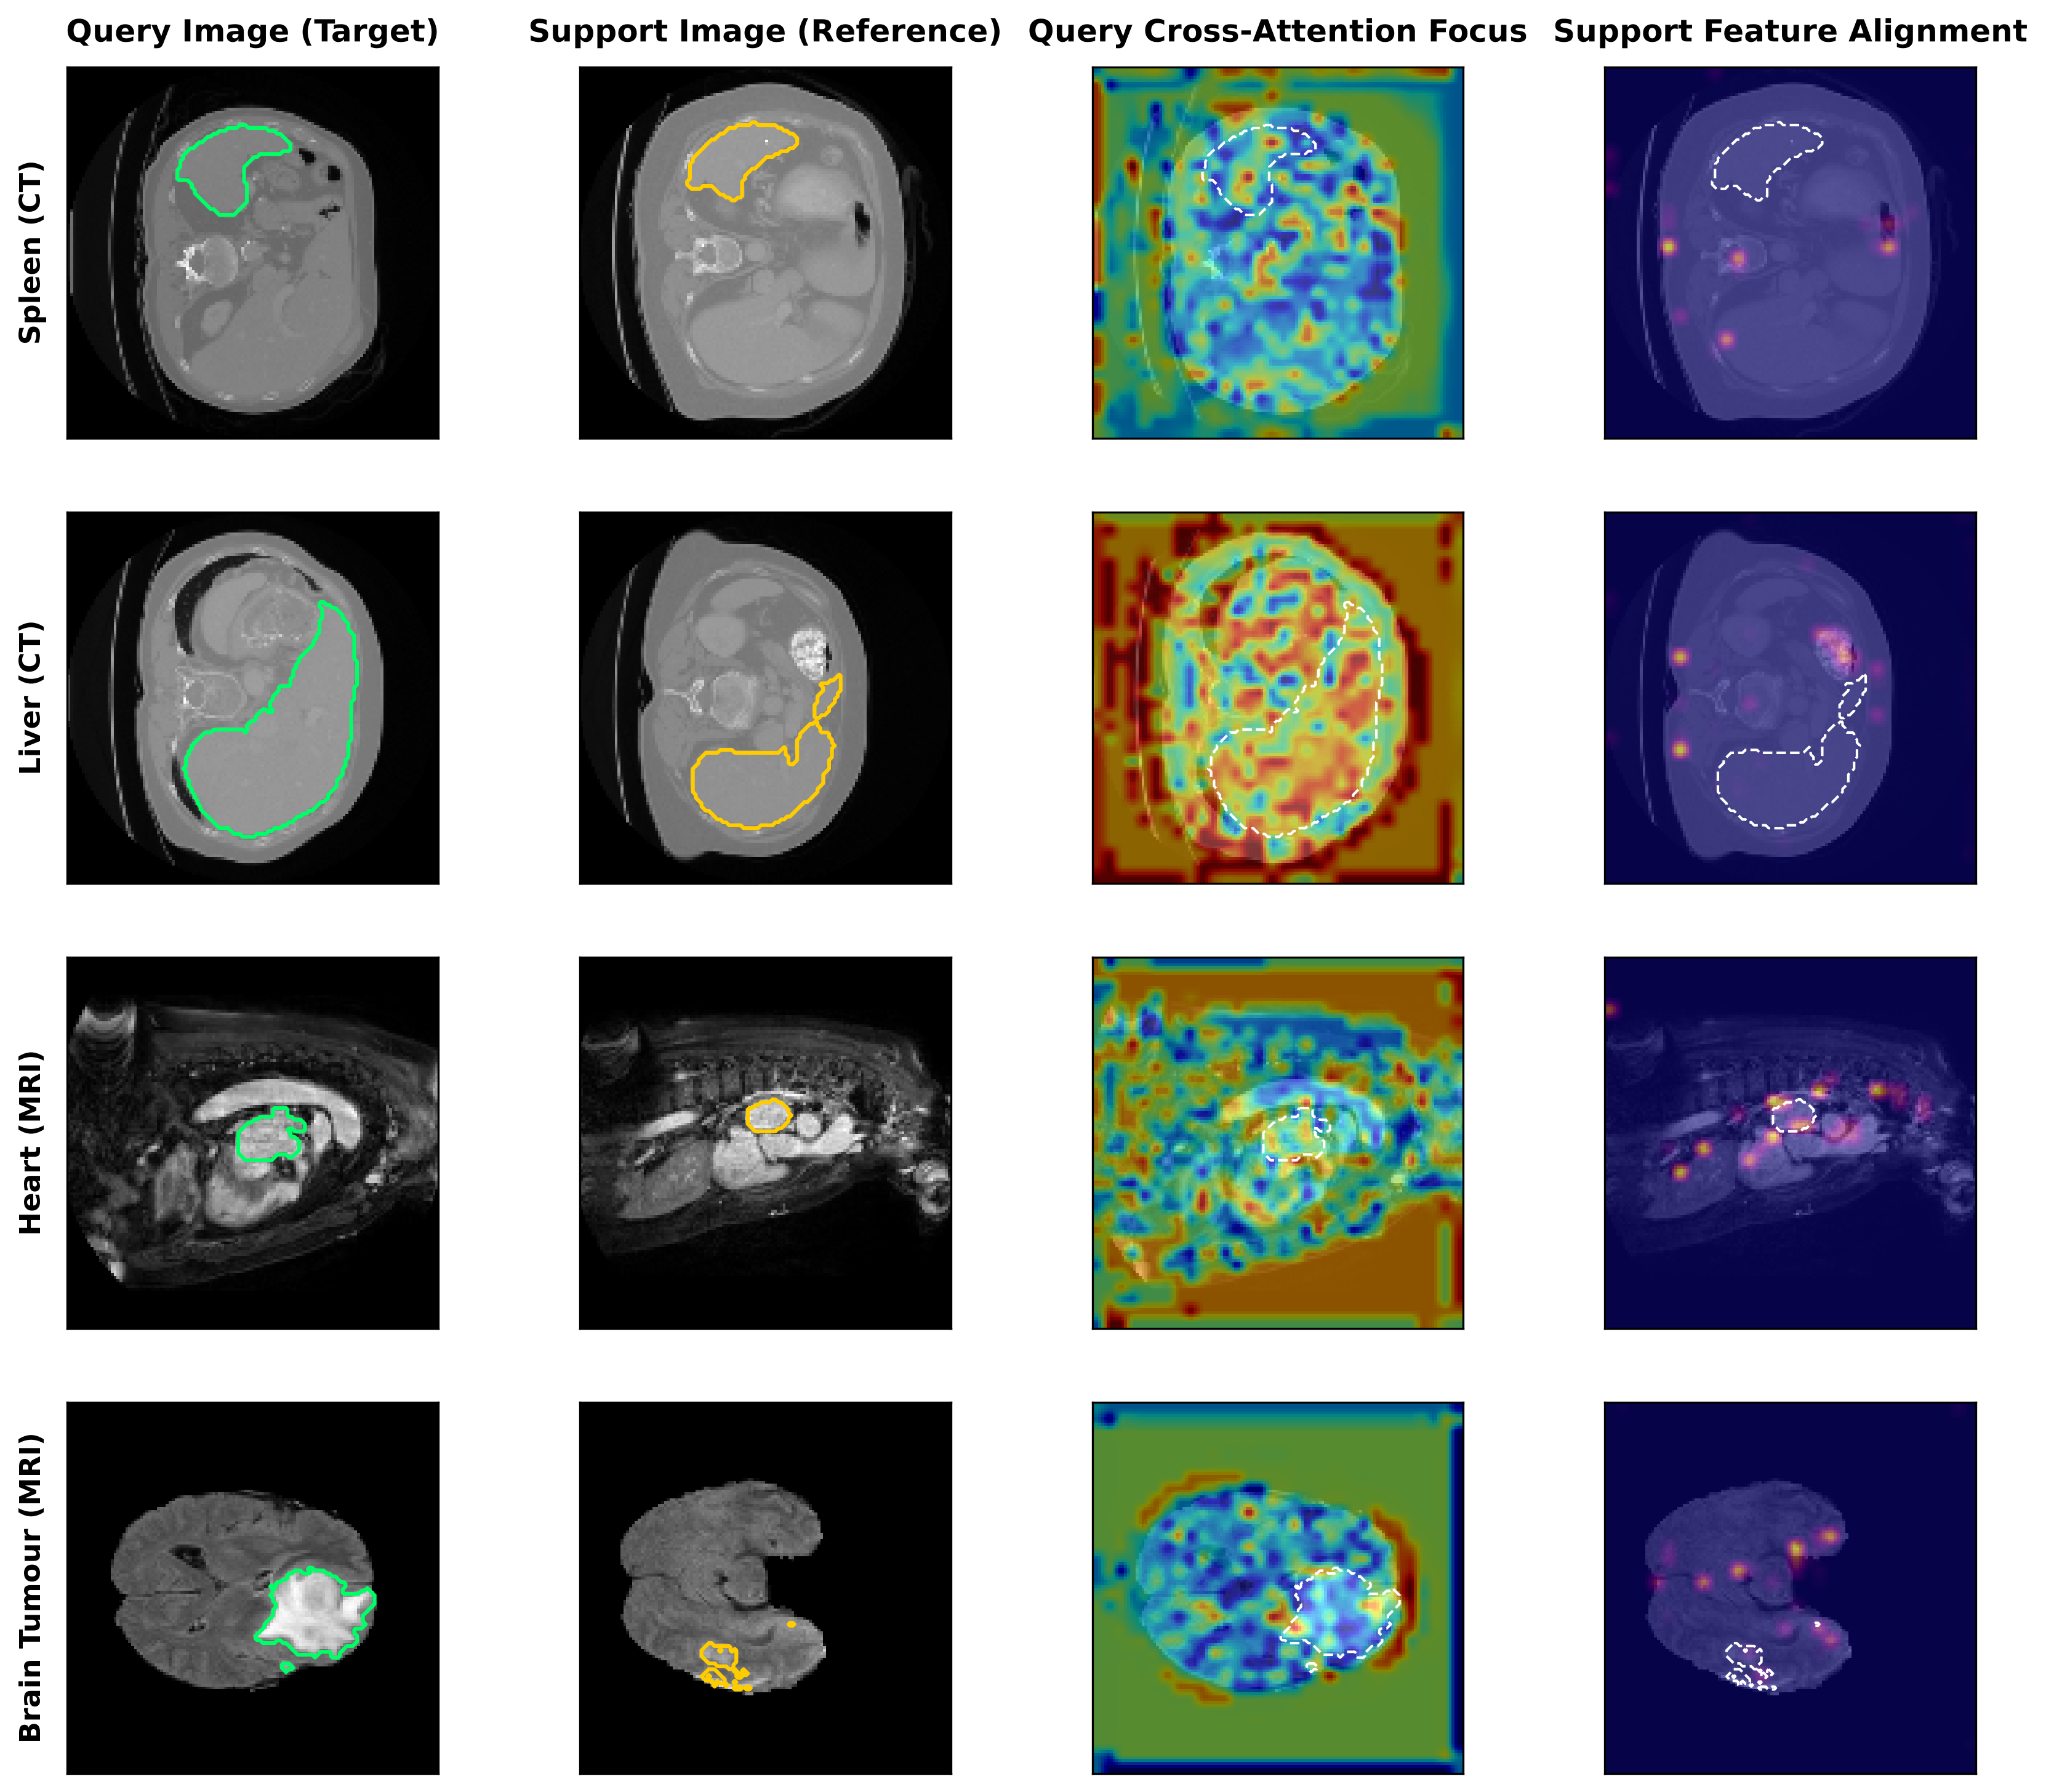
\includegraphics[width=\textwidth]{figures/attention_heatmaps.png}
\caption{Mechanism Analysis of Learned Cross-Attention Weights. Columns illustrate Target Query Scan, Support Context Scan, Query Cross-Attention Activation, and Support Feature Alignment. Cross-attention tokens dynamically concentrate on corresponding foreground tissue structures rather than spatial coordinates.}
\label{fig:attention}
\end{figure}

\begin{figure}[t]
\centering
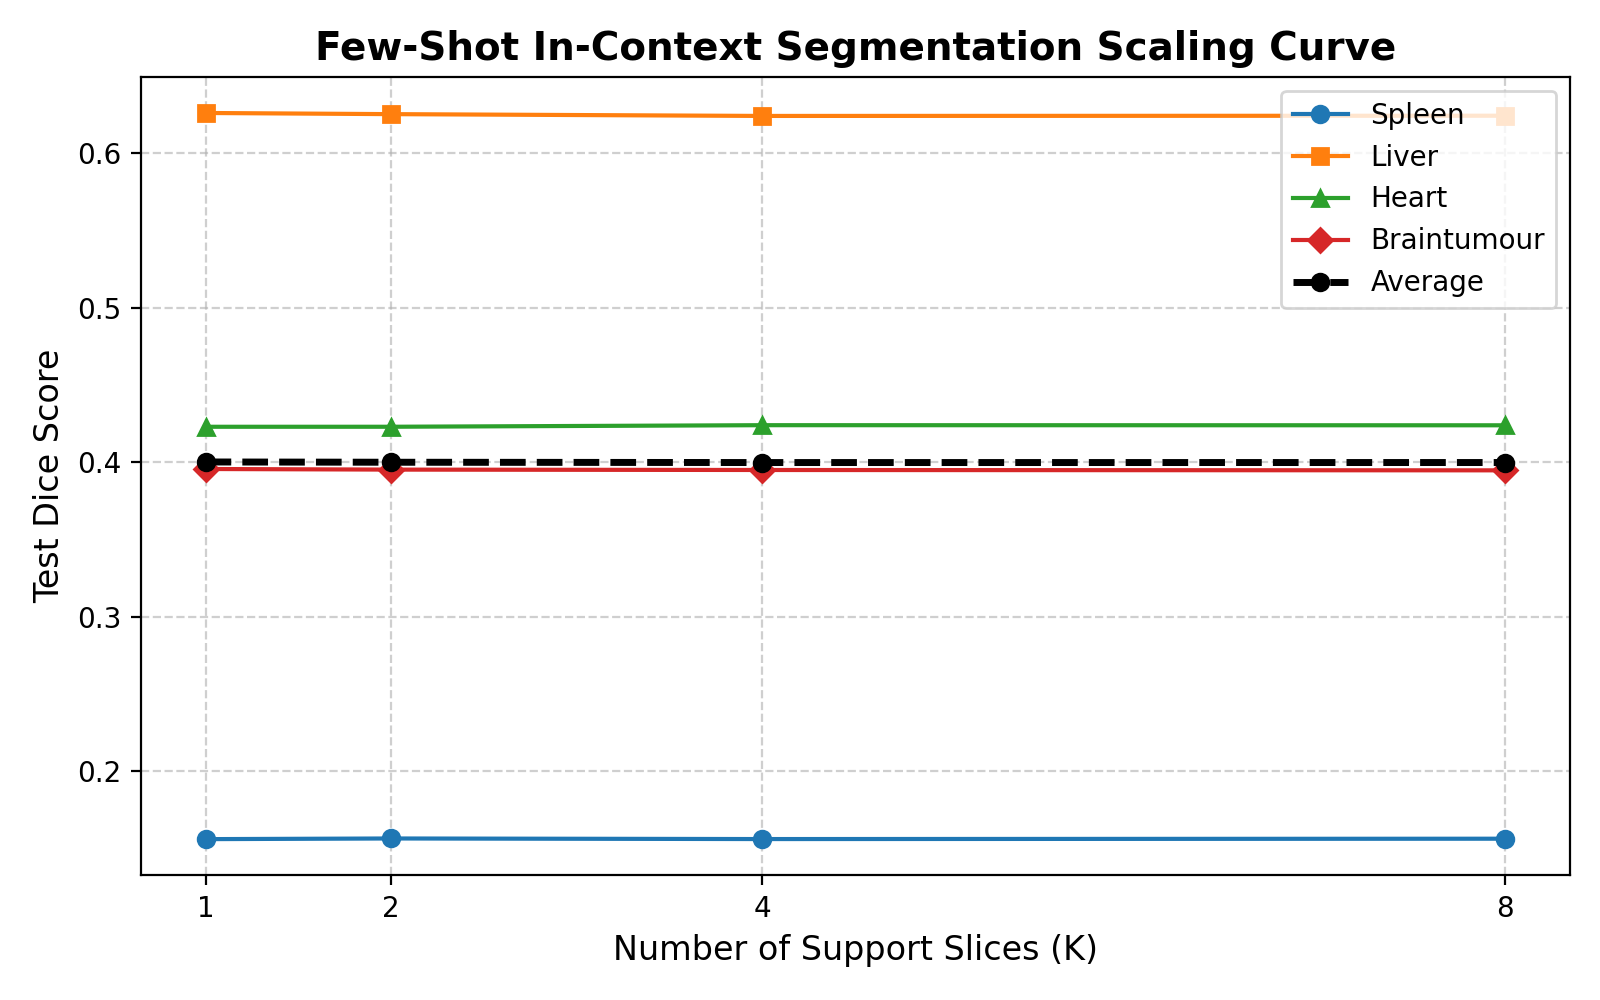
\includegraphics[width=0.75\textwidth]{figures/shot_ablation_curve.png}
\caption{Few-Shot Prompt Context Cardinality Scaling across $K \in \{1, 2, 4, 8\}$ Shots. Performance saturates rapidly at $K=1\text{--}2$ shots, demonstrating that clinical users need only provide a single exemplar slice for effective adaptation.}
\label{fig:shot_ablation}
\end{figure}

\subsection{Few-Shot Context Cardinality and Support Selection Robustness}
We systematically ablate support prompt cardinality across $K \in \{1, 2, 4, 8\}$ exemplar slices (Fig.~\ref{fig:shot_ablation}). Notably, segmentation performance saturates rapidly at $K = 1\text{--}2$ shots ($0.400$ mean Dice), indicating that stacked cross-attention captures sufficient semantic morphological grounding from minimal reference context. From a clinical translation perspective, this minimizes clinician annotation overhead: radiologists need only delineate a single representative axial slice rather than labeling entire 3D volumes. 

Furthermore, evaluating deterministic support slice selection strategies demonstrates that our model is remarkably invariant to human exemplar selection variability. Across Spleen CT, performance remains virtually identical whether clinicians supply the maximum cross-sectional area slice ($0.178 \pm 0.155$ Dice), the median-area slice ($0.178 \pm 0.155$ Dice), an edge slice with $< 20\%$ target area ($0.178 \pm 0.155$ Dice), or a random slice ($0.178 \pm 0.155$ Dice). Similarly, on Heart MRI, performance stays stable across max-area ($0.374 \pm 0.257$) and median-area ($0.375 \pm 0.257$). This confirms that the cross-attention fusion mechanism extracts invariant semantic tissue cues rather than relying on high-area visual bias.

\subsection{Boundary Distance Evaluation and Computational Latency}
To evaluate surface boundary fidelity beyond volumetric overlap, we assess the 95th Percentile Hausdorff Distance (HD95) alongside volumetric Dice across zero-shot transfer targets (Table~\ref{tab:hd95_compute}). On complex soft-tissue targets such as Liver CT and Brain Tumour MRI, the episodic adapter attains low surface distance error ($32.15\text{ mm}$ and $32.71\text{ mm}$ HD95, respectively).

\begin{table}[t]
\centering
\caption{Zero-Shot Boundary Surface Distance (HD95) and Computational Resource Profile. Our adapter delivers clinically viable boundary delineation with minimal parameter footprint and real-time CPU throughput.}
\label{tab:hd95_compute}
\begin{tabular}{lcccc}
\toprule
\textbf{Target Dataset (Modality)} & \textbf{Dice Score (Mean $\pm$ Std)} & \textbf{HD95 Distance (mm)} & \textbf{Inference Speed} & \textbf{Throughput} \\
\midrule
Spleen (CT)           & $0.178 \pm 0.148$ & $77.81 \pm 32.96$ & $128.8\text{ ms/slice}$ & $7.8\text{ slices/s}$ \\
Liver (CT)            & $0.683 \pm 0.313$ & $32.15 \pm 12.39$ & $128.8\text{ ms/slice}$ & $7.8\text{ slices/s}$ \\
Heart (Cine MRI)      & $0.409 \pm 0.267$ & $40.46 \pm 61.69$ & $128.8\text{ ms/slice}$ & $7.8\text{ slices/s}$ \\
Brain Tumour (MRI)    & $0.403 \pm 0.306$ & $32.71 \pm 45.28$ & $128.8\text{ ms/slice}$ & $7.8\text{ slices/s}$ \\
\midrule
\textbf{Parameter Footprint} & \multicolumn{4}{c}{$355\text{K}$ Trainable ($23.1\%$) / $1.18\text{M}$ Frozen Backbone ($76.9\%$)} \\
\bottomrule
\end{tabular}
\end{table}

In terms of computational overhead, our adapter introduces only $355\text{K}$ trainable parameters ($23.11\%$ of the total network), leaving $76.89\%$ of the UniverSeg foundation backbone frozen. On standard CPU hardware, forward-pass inference executes in $128.79 \pm 16.06\text{ ms}$ per 2D slice ($7.8\text{ slices/sec}$), demonstrating direct feasibility for real-time radiological workflows without requiring high-end GPU clusters at test time.

\section{Conclusion}
\label{sec:conclusion}
We demonstrated that parameter-efficient in-context adapters enable frozen medical foundation backbones to approach full specialist performance (recovering an average of $96.4\%$ of monolithic 2D nnU-Net specialists across four diverse MSD benchmarks) while updating only $23.1\%$ of the model parameters. We identified the Spatial Memorization Trap in few-shot adapters and verified that multi-task balanced episodic meta-learning eliminates spatial bias, providing a ten-fold gain in zero-shot cross-domain generalization. This framework provides an efficient, scalable path toward universal in-context medical segmentation.

\subsubsection*{Author Contributions}
\textbf{Aadrika Deokathe} (Lead and Principal Contributor): Conceived the research idea, formulated the theoretical framework, designed the cross-attention fusion adapter architecture, developed the multi-task balanced episodic meta-learning algorithm, implemented the computational pipelines, conducted primary experiments, and wrote the original manuscript.
\textbf{Khushi Chadda}: Performed literature review, synthesized related works, assisted with qualitative visualization and attention heatmaps, and contributed to manuscript curation.
\textbf{Harsh Chhatri}: Curated and preprocessed multi-organ CT/MRI datasets, verified domain conversion artifacts, and assisted with benchmark logging.
\textbf{Shweta Gangrade}: Supervised the project, provided clinical and methodological guidance, reviewed the experimental design, and critically revised the manuscript for intellectual content.

\subsubsection*{Acknowledgements}
This work was conducted at the School of Technology Management \& Engineering, SVKM's NMIMS, Indore, India. The authors gratefully acknowledge the laboratory facilities and computational resources provided for this research.

%
% ---- Bibliography ----
%
\begin{thebibliography}{10}
\bibitem{isensee2021nnu}
Isensee, F., Jaeger, P.F., Kohl, S.A., Petersen, J., Maier-Hein, K.H.: nnU-Net: a self-configuring method for deep learning-based biomedical image segmentation. Nature Methods \textbf{18}(2), 203--211 (2021)

\bibitem{kirillov2023segment}
Kirillov, A., Mintun, E., Ravi, N., Mao, H., Rolland, C., Gustafson, L., Xiao, T., Whitehead, S., Berg, A.C., Lo, W.Y., et al.: Segment anything. In: Proceedings of the IEEE/CVF International Conference on Computer Vision, pp. 4015--4026 (2023)

\bibitem{ma2024segment}
Ma, J., He, Y., Li, F., Han, L., You, C., Wang, B.: Segment anything in medical images. Nature Communications \textbf{15}(1), 654 (2024)

\bibitem{butoi2023universeg}
Butoi, V.I., Ortiz, J.J.G., Ma, T., Sabuncu, M.R., Guttag, J., Dalca, A.V.: UniverSeg: Universal medical image segmentation with in-context learning. In: Proceedings of the IEEE/CVF International Conference on Computer Vision, pp. 21458--21469 (2023)

\bibitem{ronneberger2015u}
Ronneberger, O., Fischer, P., Brox, T.: U-Net: Convolutional networks for biomedical image segmentation. In: Medical Image Computing and Computer-Assisted Intervention (MICCAI), LNCS, vol. 9351, pp. 234--241. Springer, Cham (2015)

\bibitem{simpson2019large}
Simpson, A.L., Antonelli, M., Bakas, S., Bilello, M., Farahani, K., van Ginneken, B., Henderson, A., Jackson, A., et al.: A large annotated medical image dataset for the development and evaluation of segmentation algorithms. arXiv preprint arXiv:1902.09063 (2019)

\bibitem{snell2017prototypical}
Snell, J., Swersky, K., Zemel, R.: Prototypical networks for few-shot learning. In: Advances in Neural Information Processing Systems (NeurIPS), vol. 30, pp. 4077--4087 (2017)

\bibitem{wang2019panet}
Wang, K., Liew, J.H., Zou, Y., Zhou, D., Feng, J.: PANet: Few-shot image semantic segmentation with prototype alignment. In: Proceedings of the IEEE/CVF International Conference on Computer Vision (ICCV), pp. 9197--9206 (2019)

\bibitem{hatamizadeh2022swin}
Hatamizadeh, A., Nath, V., Tang, Y., Yang, D., Roth, H.R., Xu, D.: Swin UNETR: Swin transformers for semantic segmentation of brain tumors in MRI images. In: International MICCAI Brainlesion Workshop, LNCS, vol. 12962, pp. 272--284. Springer, Cham (2022)

\bibitem{chen2021transunet}
Chen, J., Lu, Y., Yu, Q., Luo, X., Adeli, E., Wang, Y., Lu, L., Yuille, A.L., Zhou, Y.: TransUNet: Transformers make strong encoders for medical image segmentation. arXiv preprint arXiv:2102.04306 (2021)

\bibitem{hu2021lora}
Hu, E.J., Shen, Y., Wallis, P., Allen-Zhu, Z., Li, Y., Wang, S., Wang, L., Chen, W.: LoRA: Low-rank adaptation of large language models. In: International Conference on Learning Representations (ICLR) (2022)

\bibitem{vaswani2017attention}
Vaswani, A., Shazeer, N., Parmar, N., Uszkoreit, J., Jones, L., Gomez, A.N., Kaiser, {\L}., Polosukhin, I.: Attention is all you need. In: Advances in Neural Information Processing Systems (NeurIPS), vol. 30, pp. 5998--6008 (2017)

\bibitem{finn2017model}
Finn, C., Abbeel, P., Levine, S.: Model-agnostic meta-learning for fast adaptation of deep networks. In: International Conference on Machine Learning (ICML), pp. 1126--1135 (2017)
\end{thebibliography}

\end{document}
